\documentclass[11pt,letterpaper]{article}
\usepackage{xcolor}
\usepackage{textcomp,marvosym}
\usepackage{amsmath,amssymb}
\usepackage[left]{lineno}
\usepackage{changepage}
\usepackage{rotating}
\usepackage{natbib}
\usepackage{setspace}
\usepackage{fancyhdr}
\usepackage{graphicx}
\usepackage{sidecap}
\usepackage{pdfpages}
\usepackage{longtable}
\usepackage{url}

\usepackage[aboveskip=1pt,labelfont=bf,labelsep=period,justification=raggedright,singlelinecheck=off]{caption}
\doublespacing

\raggedright
\textwidth = 6.5 in
\textheight = 8.25 in
\oddsidemargin = 0.0 in
\evensidemargin = 0.0 in
\topmargin = 0.0 in
\headheight = 0.0 in
\headsep = 0.5 in
\parskip = 0.1 in
\parindent = 0.2 in

\pagestyle{myheadings}
\pagestyle{fancy}
\fancyhf{}
\lhead{Swanson-Hysell et al., Geology, doi:10.1130/G47873.1}
\rhead{\thepage}

\begin{document}

\begin{flushleft}
{\Large \textbf{Rapid emplacement of massive Duluth Complex intrusions within the Midcontinent Rift}}
\\
Nicholas L. Swanson-Hysell\textsuperscript{1}, Steven A. Hoaglund\textsuperscript{2}, James L. Crowley\textsuperscript{3}, Mark D. Schmitz\textsuperscript{3}, Yiming Zhang\textsuperscript{1}, James D. Miller Jr.\textsuperscript{2}
\\
\bigskip
\textsuperscript{1} Department of Earth and Planetary Science, University of California, Berkeley, CA, USA\\
\textsuperscript{2} Department of Earth and Environmental Sciences, University of Minnesota, Duluth, MN, USA \\
\textsuperscript{3} Department of Geosciences, Boise State University, Boise, ID, USA
\bigskip
\end{flushleft}

\linenumbers
%\pagestyle{empty}

\section*{ABSTRACT}

The Duluth Complex is one of the largest mafic intrusive complexes on Earth. It was emplaced as the Midcontinent Rift developed in Laurentia's interior during an interval of magmatism and extension from \textit{ca.} 1109 to 1084 Ma. This duration of magmatic activity is more protracted than is typical for large igneous provinces interpreted to have formed from decompression melting of upwelling mantle plumes. While the overall duration was protracted, there were intervals of more voluminous magmatism. New $^{206}$Pb/$^{238}$U zircon dates for the anorthositic and layered series of the Duluth Complex constrain these units to have been emplaced \textit{ca.} 1096 Ma in less than one million years (duration of 500,000 $\pm$ 260,000 years). Comparison of paleomagnetic data from these units with Laurentia's apparent polar wander path supports this interpretation. This rapid emplacement bears similarities to the geologically short duration of well-dated large igneous provinces. These data support hypotheses that call upon the co-location of lithospheric extension and anomalously hot upwelling mantle. This rapid magmatic pulse occurred more than 10 million years after initial magmatism following more than 20$^{\circ}$$\;$of latitudinal plate motion. A likely scenario is one in which upwelling mantle encountered the base of Laurentian lithosphere and flowed via ``upside-down drainage'' to locally thinned lithosphere of the Midcontinent Rift.

\section*{INTRODUCTION}

The Midcontinent Rift represents a protracted tectonomagmatic event in the interior of Laurentia (the North American craton). Voluminous outpouring of lava and emplacement of intrusions accompanied rift development (Fig. \ref{fig:map}). Magmatic activity initiated \textit{ca.} 1109 Ma and continued until \textit{ca.} 1084 Ma \citep{Swanson-Hysell2019a}. Preserved thicknesses of the volcanic successions range from nearly 10 km for partial sections exposed on land, \citep{Green2011a}, to $\sim$25 km under Lake Superior \citep{Cannon1992b}. These volcanics and associated intrusions are much more voluminous than is typical for tectonic rifting. Analysis of seismic data leads to an estimate that total eruptive volume exceeded 2 x 10$^6$ km$^3$ with a greater volume added to the lithosphere as intrusions and a magmatic underplate \citep{Cannon1992b}. The $\sim$25 Myr duration of Midcontinent Rift volcanism is much longer than is typical for large igneous province emplacement associated with decompression melting of an upwelling mantle plume. Well-dated large igneous provinces, such as the Central Atlantic Magmatic Province \citep{Blackburn2013a}, the Karoo-Ferrar large igneous province\citep{Burgess2015a}, and the Deccan Traps \citep{Schoene2019a, Sprain2019a} have durations of $<$1 Myr for the bulk of their magmatism. An explanation for prolonged volcanism in the Midcontinent Rift could attribute rift initiation and initial volcanism to plume arrival with continued volcanism resulting from rift-driven asthenospheric upwelling. However, the most voluminous period of magmatism occurred more than 10 million years after initial flood volcanism during an interval known as the ``main magmatic stage'' \citep{Vervoort2007a}. Main stage magmatism has been attributed to an upwelling mantle plume based on the large volume and geochemical signatures \citep{Nicholson1990a, White1995a}.

\begin{figure}[!ht]
\noindent\includegraphics[width=\textwidth]{./Figures/Duluth_Complex_map.pdf}
\centering
\caption{\small{Geologic map of NE Minnesota (simplified from \citealp{Jirsa2011a}) highlighting Midcontinent Rift intrusive complexes and geochronology sample locations. Volcanic and intrusive units dip towards Lake Superior typically at 10\textdegree$\;$to 20\textdegree. U-Pb dates from the anorthositic and layered series of the Duluth Complex (light and dark blue) indicate rapid emplacement in less than 1 million years.}}
\label{fig:map}
\end{figure}

Pioneering Midcontinent Rift geochronology utilized $^{207}$Pb/$^{206}$Pb dates on zircon from volcanics \citep{Davis1997a} and intrusions \citep{Paces1993a} to illuminate the magmatic history. Subsequent advances in U-Pb geochronology enable higher precision $^{206}$Pb/$^{238}$U dates to be used when chemical abrasion methods have mitigated Pb loss \citep{Mattinson2005a}.  U-Pb dates developed using these methods have led to an updated chronostratigraphic framework for Midcontinent Rift volcanics (\citealp{Swanson-Hysell2019a}; Fig. \ref{fig:dates}). With these higher precision constraints, the timing and tempo of magmatic activity within the rift can be reevaluated -- was it continuous or punctuated by pulses? Key to evaluating this question is the timing of emplacement of intrusive rocks, particularly the largest intrusive suite -- the Duluth Complex (Fig. \ref{fig:map}). With its arcuate area of 5630 km$^2$, the tholeiitic Duluth Complex is the second-largest exposed mafic intrusive complex on Earth \citep{Miller2002c}. It was emplaced as sheet-like intrusions into the base of a comagmatic volcanic succession with the majority of its volume associated with the anorthositic series and the layered series of gabbroic and troctolitic cumulates (\citealp{Miller2002c}; Fig. \ref{fig:map}). We present $^{206}$Pb/$^{238}$U zircon dates from the Duluth Complex, as well as the Beaver Bay Complex (Fig. \ref{fig:map}), to improve constraints on the duration of intrusive magmatism and contextualize it with the chronology of volcanism.

\section*{METHODS and RESULTS}

Zircon crystals were chemically abraded prior to analysis by isotope dilution thermal ionization mass spectrometry (ID-TIMS).\footnote{Supplemental Material. Individual zircon dates, paleomagnetic site mean directions, and additional method details. Please visit https://doi.org/10.1130/G47873.1 to access the supplemental material, and contact editing@geosociety.org with any questions. Paleomagnetic data and interpreted directions are available in the Magnetics Information Consortium (MagIC) database (\url{https://earthref.org/MagIC/doi/10.1130/G47873.1}). Geochronological data are available at https://www.geochron.org associated with International Geosample Numbers (IENSH000H, IENSH000I, IENSH000J, IENSH000K, IENSH000L and IENSH000M). Code associated with statistical tests and data visualization is available in a Zenodo repository \url{https://zenodo.org/}).} Weighted means were calculated from multiple single zircon dates (Fig. \ref{fig:dates} and Table \ref{tab:geochron}). These $^{206}$Pb/$^{238}$U dates can be compared to one another, and to the volcanic dates of \cite{Swanson-Hysell2019a}, at the level of analytical uncertainty (X uncertainty in Table \ref{tab:geochron}) given that all dates were developed using EARTHTIME tracer solutions \citep{Condon2015a}. This 2$\sigma$ analytical uncertainty will be reported when dates are discussed. External uncertainties and mean squared weighted deviation (MSWD) values are reported in Table \ref{tab:geochron}.

The Duluth Complex anorthositic series comprises plagioclase-rich gabbroic cumulates varying from anorthositic gabbro to anorthosite. Samples FC1 and FC4b are from gabbroic anorthosite exposures near the former logging town of Forest Center (Minnesota). A weighted mean $^{206}$Pb/$^{238}$U date for FC1 of 1095.81 $\pm$ 0.16 Ma is calculated based on 10 single zircon dates (Table \ref{tab:geochron}). This date is indistinguishable from a weighted mean $^{206}$Pb/$^{238}$U date for FC1 of 1095.97 $\pm$ 0.22 Ma developed by \cite{Ibanez-Mejia2019a}. Our new FC4b date is indistinguishable from these FC1 dates with a weighted mean $^{206}$Pb/$^{238}$U date of 1095.69 $\pm$ 0.18 Ma based on dates from 7 zircons. These dates are indistinguishable from the weighted mean $^{206}$Pb/$^{238}$U date of 1095.86 $\pm$ 0.19 Ma developed from chemically-abraded zircons of anorthositic series sample AS3 collected in the city of Duluth (\citealp{Schoene2006a}; Fig. \ref{fig:dates}, Table \ref{tab:geochron}). Zircon grains from these anorthositic series samples are commonly used as U-Pb standards.

The layered series of the Duluth Complex is a suite of stratiform troctolitic to gabbroic cumulates emplaced as discrete intrusions (Fig. \ref{fig:map}). The PRI sample is an augite troctolite from the Partridge River intrusion which is at the base of the complex in contact with underlying Paleoproterozoic metasedimentary rocks (Fig. \ref{fig:map}). Data from 6 zircons result in a weighted mean $^{206}$Pb/$^{238}$U date of 1096.19 $\pm$ 0.19 Ma (Fig. \ref{fig:dates}). The BEI sample is an olivine gabbro from the Bald Eagle intrusion. This intrusion has been interpreted as one of the youngest layered series units based on cross-cutting relationships inferred from aeromagnetic data \citep{Miller2002c}. Dates from 6 zircons of BEI result in a weighted mean $^{206}$Pb/$^{238}$U date of 1095.89 $\pm$ 0.19 Ma (Fig. \ref{fig:dates}).

\begin{figure}[!ht]
\noindent\includegraphics[width=\textwidth]{./Figures/MCR_Dates.pdf}
\caption{\small{Date bar plot of CA-ID-TIMS $^{206}$Pb/$^{238}$U zircon dates for Midcontinent Rift volcanics and intrusives. Dates for volcanics and BBC-SBA1 are from \cite{Fairchild2017a} and \cite{Swanson-Hysell2019a}. The AS3 date is from \cite{Schoene2006a}. Each vertical bar represents the date for an individual zircon while the horizontal lines and grey boxes represent the weighted means and their uncertainty. The dates are colored by the geomagnetic polarity recorded by the unit or sequence of lavas. NSVG --North Shore Volcanic Group; Volcs. -- Volcanics.}}
\label{fig:dates}
\end{figure}

The Beaver Bay complex is a suite of dominantly hypabyssal intrusions that cross-cut the North Shore Volcanic Group (Fig. \ref{fig:map}). Sample HCT is an augite troctolite from the Houghtaling Creek troctolite macrodike \citep{Miller2001a}. In contrast to the internally-consistent dates from the layered and anorthositic series samples, $^{206}$Pb/$^{238}$U zircon dates from HCT have more dispersion that we interpret as resulting from Pb loss not fully mitigated by chemical abrasion. After excluding individual dates that trend away from concordia, dates from 4 concordant zircons result in a weighted mean $^{206}$Pb/$^{238}$U date of 1095.44 $\pm$ 0.26 Ma (Fig. \ref{fig:dates}). A sample of ferrodiorite was collected as WLFG from the Wilson Lake ferrogabbro of the Beaver Bay Complex. This plug-shaped zoned intrusion was emplaced into the Duluth Complex roof zone. Variable intensity chemical abrasion was applied to WLFG zircons with hotter and longer dissolution yielding more concordant data with older $^{206}$Pb/$^{238}$U dates (Table S1 in the Supplemental Material). After excluding those interpreted to have unmitigated Pb loss, dates from 5 zircons result in a weighted mean $^{206}$Pb/$^{238}$U date of 1091.63 $\pm$ 0.35 Ma (Fig. \ref{fig:dates}). This date is indistinguishable from the 1091.61 $\pm$ 0.14 Ma $^{206}$Pb/$^{238}$U date developed from an aplite within a Silver Bay intrusion of the Beaver Bay Complex (sample BBC-SBA1 of \citealp{Fairchild2017a}; Figs. \ref{fig:map} and \ref{fig:dates}).

\begin{table}[h!]
\footnotesize
\caption{Summary of CA-ID-TIMS $^{206}$Pb/$^{238}$U dates from Midcontinent Rift intrusions}
\begin{tabular}{|p{3.2 cm}|p{2.4 cm}|p{1.8 cm}|c|ccc|c|c|}
\hline
Sample & Group & Latitude & $^{206}$Pb/$^{238}$U & \multicolumn{3}{|c|}{Uncertainty (2$\sigma$)} & MSWD & n/N \\
 &  & Longitude & date (Ma) & X & Y & Z & & \\
\hline
PRI \textit{Partridge River Intrusion augite troctolite} & Duluth Complex (layered series) & 47.5480$^{\circ}$ N 92.1074$^{\circ}$ W & 1096.19 & 0.19 & 0.36 & 1.15 & 0.45 & 6/6 \\
\hline
BEI \textit{Bald Eagle Intrusion olivine gabbro} & Duluth Complex (layered series) & 47.7516$^{\circ}$ N 91.5680$^{\circ}$ W & 1095.89 & 0.19 & 0.36 & 1.15 & 1.59 & 6/6 \\
\hline
AS3 \textit{Duluth gabbroic anorthosite} & Duluth Complex (anorthositic series) & 46.7621$^{\circ}$ N 92.1590$^{\circ}$ W & 1095.86 & 0.19 & 0.36 & 1.15 & 0.43 & 8/8 \\
\hline
FC1 \textit{Forest Center gabbroic anorthosite} & Duluth Complex (anorthositic series) & 47.7827$^{\circ}$ N 91.3266$^{\circ}$ W & 1095.81 & 0.16 & 0.34 & 1.14 & 1.44 & 10/10 \\
\hline
FC4b \textit{Forest Center gabbroic anorthosite} & Duluth Complex (anorthositic series) & 47.7677$^{\circ}$ N 91.3753$^{\circ}$ W & 1095.69 & 0.18 & 0.35 & 1.14 & 0.34 & 7/8 \\
\hline
HCT \textit{Houghtaling Creek Troctolite} & Beaver Bay Complex & 47.6009$^{\circ}$ N 91.1497$^{\circ}$ W & 1095.44 & 0.26 & 0.40 & 1.16 & 1.13 & 4/11  \\
\hline
WLFG \textit{Wilson Lake Ferrogabbro ferrodiorite} & Beaver Bay Complex & 47.6620$^{\circ}$ N 91.0619$^{\circ}$ W & 1091.63 & 0.35 & 0.46 & 1.18 & 0.74 & 5/8 \\
\hline
BBC-SBA1 \textit{Silver Bay aplite} & Beaver Bay Complex & 47.6620$^{\circ}$ N 91.0619$^{\circ}$ W & 1091.61 & 0.14 & 0.30 & 1.2 & 1.0 & 6/6 \\
\hline
\end{tabular}\\
%\begin{tablenotes}[para,flushleft]
Notes: X is 2$\sigma$ analytical uncertainty; Y is 2$\sigma$ uncertainty also incorporating tracer calibration for comparison to U-Pb dates not developed using EARTHTIME-calibrated tracer solutions; Z is 2$\sigma$ uncertainty including X and Y, as well as $^{238}$U decay constant uncertainty (0.108$\%$; \citealp{Jaffey1971a}). This Z uncertainty needs to be utilized when comparing to dates using other decay systems (e.g., $^{40}$Ar/$^{39}$Ar, $^{187}$Re-$^{187}$Os); MSWD is the mean squared weighted deviation; n is the number of individual zircon dates included in the calculated sample mean date; N is the number of individual zircons analyzed for the sample. All dates are from this study with the exceptions of samples AS3 \citep{Schoene2006a} and BBC-SBA1 \citep{Fairchild2017a}.
%\end{tablenotes}
\label{tab:geochron}
\end{table}

Paleomagnetic data from the layered series (37 sites) and the anorthositic series (11 sites) near Duluth were published in \cite{Beck1970a} (Fig. \ref{fig:poles}). Site directions of the layered and anorthositic series share a common mean, consistent with their overlapping U-Pb dates. In order to pair paleomagnetic data with geochronology, oriented cores were collected and analyzed from the sites of FC1, FC4 and HCT. Magnetization was measured on a 2G DC-SQUID magnetometer at UC Berkeley. Samples underwent alternating field (AF) or thermal demagnetization steps and fits were made using PmagPy software \citep{Tauxe2016a}. While \cite{Beck1970a} did not implement tilt corrections, the Duluth Complex and overlying lavas dip towards Lake Superior and paleomagnetic data need to be corrected for this tilt. We compile abundant igneous layering orientations, which are similar to the tilt of overlying lavas and interflow sediments, and use them for tilt correction.

\begin{figure}[!ht]
\noindent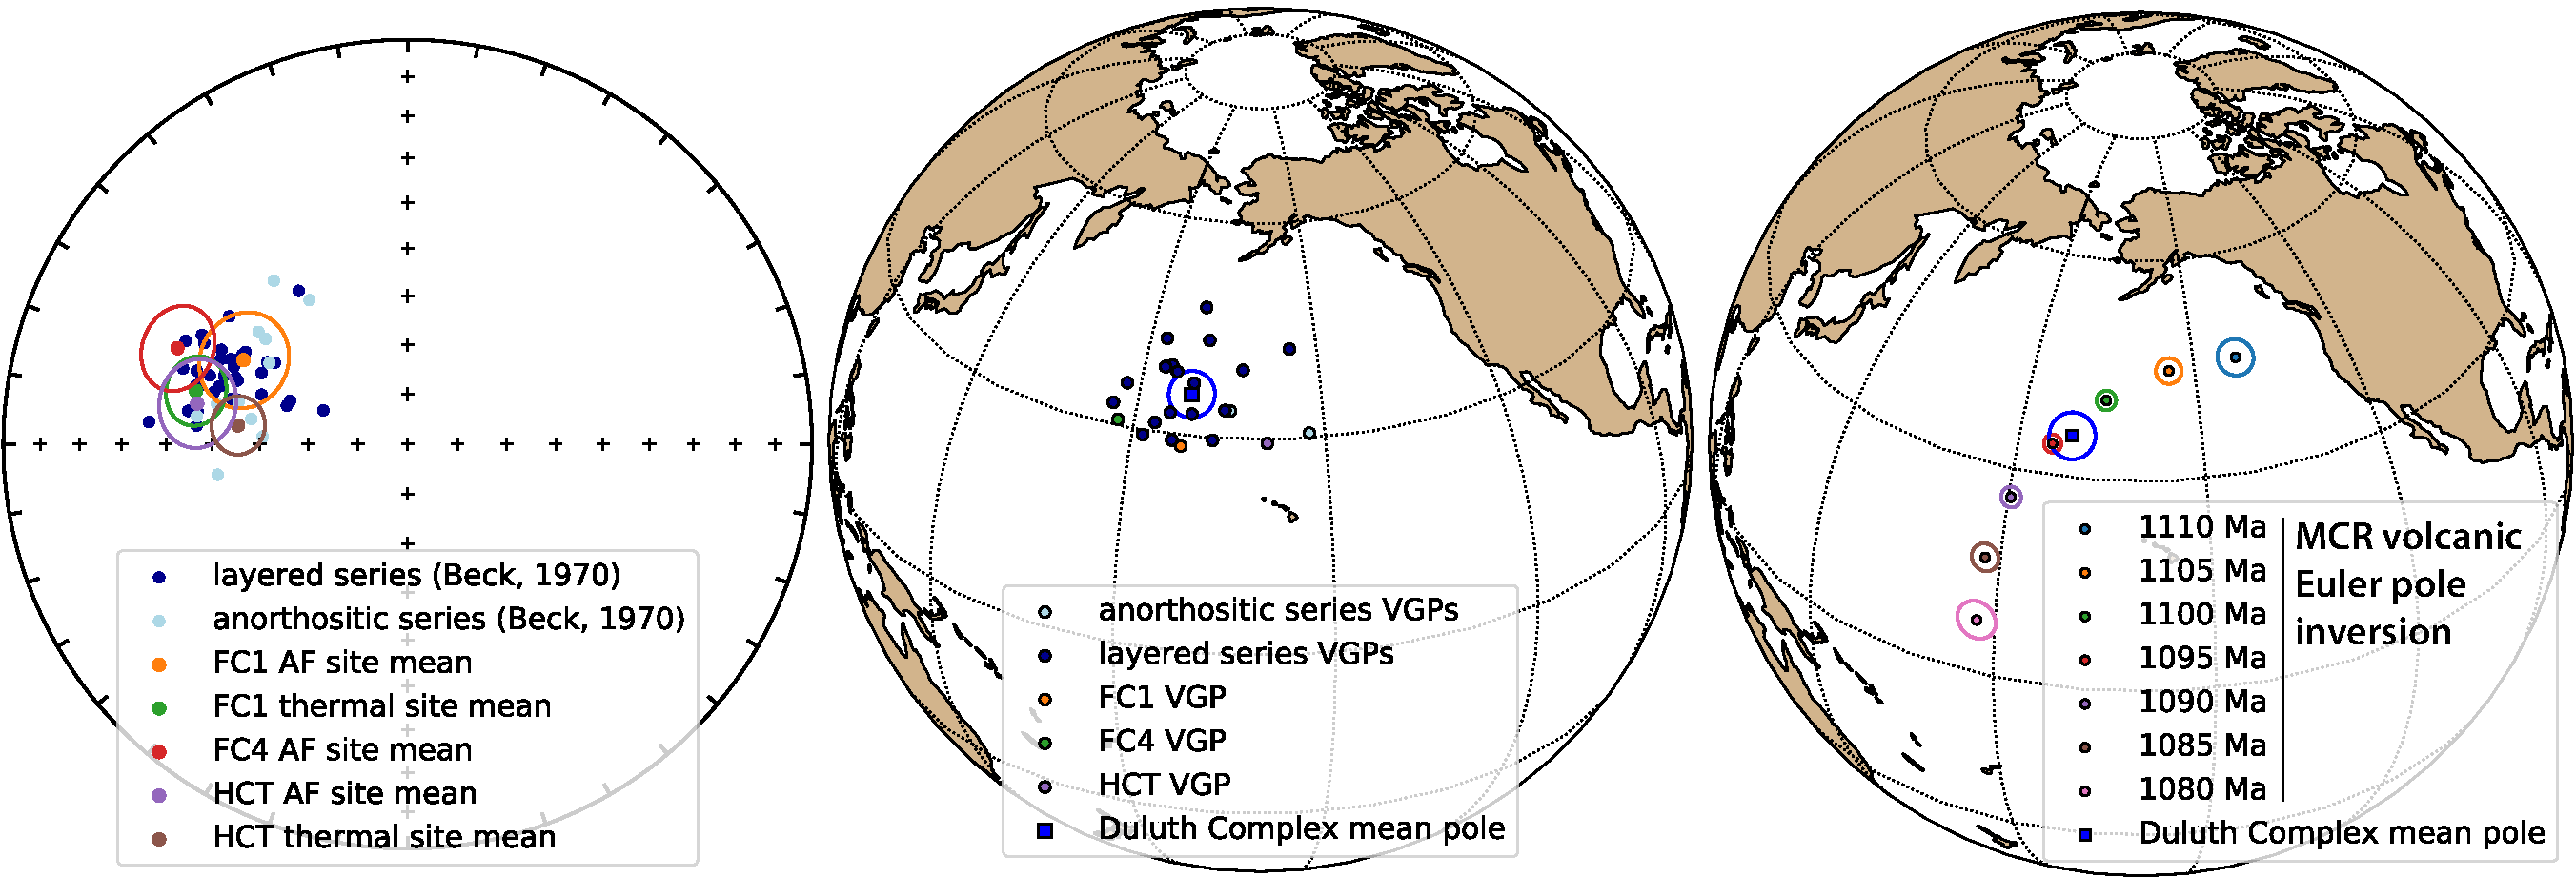
\includegraphics[width=\textwidth]{./Figures/Duluth_Complex_pole.pdf}
\caption{\small{Left panel: tilt-corrected site mean paleomagnetic directions from anorthositic and layered series sites of \cite{Beck1970a} and from the FC1, FC4, and HCT sites. Center panel: Virtual geomagnetic poles (VGPs) for sites with 95$\%$ confidence angle $\alpha_{95}<15^{\circ}$ give a mean pole of: 188.7$^{\circ}$ E, 35.6$^{\circ}$ N, N=24, A$_{95}$=3.1, k=92. Right panel: Duluth Complex pole shown with a synthesized pole path developed from Midcontinent Rift (MCR) volcanic poles.}}
\label{fig:poles}
\end{figure}

Rapid progression of poles within the apparent polar wander path (APWP) enable these paleomagnetic data to give chronological insight. Pole positions from the early stage of rift magmatism are different from those of main stage lavas (Fig. \ref{fig:poles}). The similar position of Duluth Complex layered and anorthositic series virtual geomagnetic poles (VGPs) is consistent with contemporaneous emplacement and they can be combined into a mean pole (Fig. \ref{fig:poles}). This pole can be compared to a synthesized APWP developed using an Euler pole inversion of chronostratigraphically-controlled volcanic poles \citep{Swanson-Hysell2019a}. The Duluth Complex pole lies between the 1100 Ma and 1095 Ma path positions with the $A_{95}$ uncertainty of the pole overlapping with the two angular standard deviations ellipse of the 1095 Ma path position. This result is consistent with a \textit{ca.} 1096 Ma age for the layered and anorthositic series and strengthens the correlation with the volcanics.

\section*{DISCUSSION}

Our new U-Pb dates, together with paleomagnetic data, imply that the bulk of the Duluth Complex layered series and anorthositic series were emplaced in less than 1 million years. The age differences between the anorthositic series and BEI layered series dates are all within uncertainty of no difference. The Partridge River intrusion layered series date is slightly older with an age difference from the rest of the anorthositic and layered series dates that is distinct from zero at 95$\%$ confidence. Taking this oldest date of 1096.19 $\pm$ 0.19 Ma for PRI and the youngest date of 1095.69 $\pm$ 0.18 Ma from FC4b yields a duration of overall emplacement of the layered and anorthositic series of 500,000 $\pm$ 260,000 years (2$\sigma$).  This emplacement was coeval with eruption of the North Shore Volcanic Group (NSVG) upper southwest sequence which comprises $\sim$7900 meters of lavas and is the thickest exposed Midcontinent Rift volcanic succession (Fig. \ref{fig:map}; \citealp{Green2011a,Swanson-Hysell2019a}). This rapid emplacement of the bulk of the Duluth Complex, together with coeval NSVG eruptions, require a large pulse of melt generation \textit{ca.} 1096 Ma.

%The data therefore confirm the interpretation of a geologically-short duration of peak intrusive activity made by \cite{Paces1993a} on the basis of 4 $^{207}$Pb/$^{206}$Pb dates that can be interpreted to constrain the duration to be less than 1.3 million years at 95$\%$ confidence.

%Our new $^{206}$Pb/$^{238}$U dates from the Duluth Complex layered and anorthositic series can be compared with those from the volcanic succession to constrain that t

The 1095.44 $\pm$ 0.26 Ma age of the Houghtaling Creek troctolite is indistinguishable from the youngest Duluth Complex anorthositic series date. This result indicates that this pulse of voluminous magmatic activity is represented in some Beaver Bay Complex intrusions. A younger pulse of Beaver Bay Complex magmatism postdates NSVG eruptions, evidenced by units such as the Silver Bay intrusions penetrating the youngest NSVG lavas, including the 1093.94 $\pm$ 0.28 Ma Palisade Rhyolite (\citealp{Miller2001a, Swanson-Hysell2019a}; Fig. \ref{fig:map}). The age of this magmatism is constrained by indistinguishable dates of 1091.63 $\pm$ 0.35 Ma for the Wilson Lake ferrogabbro and 1091.61 $\pm$ 0.14 Ma from the Silver Bay intrusions (Fig. \ref{fig:dates}; Table \ref{tab:geochron}). This younger Beaver Bay Complex magmatism is coeval with eruption of the $>$5 km thick Portage Lake Volcanics that are exposed to the east on the Keweenaw Peninsula and Isle Royale in Michigan (Fig. \ref{fig:dates}).

Rapid emplacement of the voluminous layered and anorthositic series of the Duluth Complex bears similarities to the geologically short duration ($<$1 Myr) of well-dated flood basalt provinces \citep{Burgess2015a, Schoene2019a}. This similarity supports the hypothesis put forward by \cite{Green1983a}, and advanced by others including \cite{Cannon1992a} and \cite{Stein2015a}, that co-location of massive magmatism and rifting is the result of lithospheric extension atop decompression melting of an upwelling mantle plume. Contemporaneous heating of Laurentia lithosphere 600 km to the north of the rift is indicated by thermochronologic data from middle to lower crustal xenoliths \citep{Edwards2018a}. Basaltic magma was also emplaced throughout the Southwestern Laurentia large igneous province coeval with rift magmatism, including sills $>$2300 km to the southwest of Duluth \citep{Bright2014a}. That such a broad region of Laurentia lithosphere experienced heating and magmatism supports hypothesized large-scale mantle upwelling.

%The Nd and Re-Os isotopic signatures of lava flows have been interpreted to be the result of plume-derived melts with variable interaction with continental lithospheric mantle \citep{Nicholson1997a, Shirey1997a}.

Both the \textit{ca.} 1108 Ma early stage and \textit{ca.} 1096 Ma main stage magmatic intervals within the Midcontinent Rift were voluminous and have been interpreted to be the result of a plume-related thermal anomaly. The interpretation that this volcanism is associated with a deep-seated mantle plume needs to be reconciled with the long duration of magmatism and rapid equatorward motion of Laurentia from a latitude of $\sim$54$^{\circ}$ N \textit{ca.} 1108 Ma during early stage flood basalt eruptions to $\sim$32$^{\circ}$ N by \textit{ca.} 1096 Ma (paleolatitudes for Duluth, MN). While some motion could be associated with true polar wander, in which the mesosphere and asthenosphere rotated in conjunction with the lithosphere,  paleomagnetic pole positions require a substantial component of plate tectonic motion \citep{Swanson-Hysell2019a}. The pulsed nature of magmatic activity could support an interpretation of multiple upwelling pulses. As postulated by \cite{Cannon1992a}, the initial pulse expressed by \textit{ca.} 1108 early stage flood basalt volcanism initiated lithospheric thinning. Given the significantly thinned lithosphere in the Midcontinent Rift region, subsequent positively-buoyant plume material that encountered Laurentia lithosphere would have experienced ``upside-down'' drainage wherein relief at the base of the lithosphere resulted in lateral and upward flow into the Midcontinent Rift \citep{Sleep1997a, Swanson-Hysell2014b}. Flow of upwelling mantle to locally-thin lithosphere would have led to ponding and concentrated decompression melting within the rift. One scenario is that Laurentia was migrating over a plume generation zone \citep{Burke2008a} from which multiple deep-seated mantle plumes upwelled and reached the lithosphere during rift development. The first could have been centered on the present-day Lake Superior region with the second encountering Laurentian lithosphere and being directed to the rift by upside-down drainage in addition to driving magmatism in southwest Laurentia. Another scenario is that \textit{ca.} 1096 Ma magmatism was invigorated by upwelling return flow enhanced by slab avalanche induced downwelling connected to the rapid plate motion of Laurentia that initiated in the early stage \citep{Swanson-Hysell2019a}. Overall, the constraint that both the anorthositic and layered series of the Duluth Complex were emplaced in less than 1 million years requires an exceptional thermal anomaly that led to rapid and voluminous melt generation during the main stage of Midcontinent Rift development.

%The indistinguishable age of rocks from the anorthositic and layered series of the Duluth Complex continue to support the model where they are genetically linked to the same episode of melt generation. The main variability between the two nearly-coeval intrusive suites comes in the concentration of plagioclase crystals with contact relationships suggesting that the crystal-ladened melts of the anorthositic complex being emplaced prior to less crystal-rich magma of the layered series intrusions \citep{Miller2002c}.

%Including a discussion of other examples of co-located massive basaltic volcanism and rifting here could be valuable: CAMP; North Atlantic; Afar

\subsection*{ACKNOWLEDGEMENTS}
Project research was supported by U.S. National Science Foundation (NSF) grant EAR-1847277 (to NLS-H) and the University of Minnesota Duluth. Funding for Boise State Isotope Geology Laboratory analytical infrastructure was provided by NSF grants EAR-0824974 and EAR-0521221. Margaret Avery and Dan Costello provided field assistance. Constructive reviews by Mauricio Iba\~nez-Mejia, Kyle Samperton, and an anonymous reviewer improved the manuscript.
\footnotesize

%Insights from Noah McLean improved the presentation of date comparisons and associated uncertainty.

\singlespacing

\bibliographystyle{gsabull}
\bibliography{../../../0000_Github/references/allrefs}

\end{document}
